
\documentclass[aspectratio=169]{beamer}
\usetheme{metropolis}           % Use metropolis theme
\usepackage[utf8]{inputenc}
\usepackage{graphicx}
\usepackage{eso-pic}
\usepackage{graphics}
\usepackage{tikz}
\usepackage[export]{adjustbox}
\usepackage{multicol}
\usepackage{listings}
\usepackage{helvet}
\usepackage{booktabs}
\usepackage{threeparttable}
\usepackage{fontspec}
\usepackage{hyperref}
\hypersetup{urlcolor=DarkBlue}

\title{Topic 6 - Track 1 \newline Descriptive Statistics:
\newline Creating Tables}
\date{\today}
\author{Author of Session here!} % Name of author(s) of session here
\institute{Development Impact Evaluation (DIME) \newline The World Bank }
\setbeamercolor{background canvas}{bg=white}	% Sets background color

% The below command places the World Bank logo and DIME logo to the right corner
\titlegraphic{%
	\begin{picture}(0,0)
	\put(330,-180){\makebox(0,0)[rt]{
\includegraphics[width=3cm]{../../img/WB_logo}}}
	\end{picture}%
	\begin{picture}(0,0)
	\put(390,-180){\makebox(0,0)[rt]{
\includegraphics[width=1.5cm]{../../img/i2i}}}
	\end{picture}%
}

%%% Section page with picture of Light bulb
\makeatletter
\defbeamertemplate*{section page}{mytheme}[1][]{
	\centering
	\begin{minipage}{22em}
		\raggedright
		\usebeamercolor[fg]{section title}
		\usebeamerfont{section title}
		\par
		\ifx\insertsubsectionhead\@empty\else%
		\usebeamercolor[fg]{subsection title}%
		\usebeamerfont{subsection title}%
		\fi
		\ifstrempty{#1}{}{%
			\includegraphics[width=100mm, height=60mm]{#1}%
		}
		\insertsectionhead\\[-1ex]
		\insertsubsectionhead
		\usebeamertemplate*{progress bar in section page}

	\end{minipage}
	\par
	\vspace{\baselineskip}
}
\makeatother

%%% Define a command to include picture in section,
%%% make section, and revert to old template
\newcommand{\sectionpic}[2]{
	\setbeamertemplate{section page}[mytheme][#2]
	\section{#1}
	\setbeamertemplate{section page}[mytheme]
}

%%% The command below allows for the text that contains Stata code
\lstset{ %
	backgroundcolor=\color{white},
	basicstyle=\tiny,
	breakatwhitespace=false,
	breaklines=true,
	captionpos=b,
	commentstyle=\color{mygreen},
	escapeinside={\%*}{*)},
	extendedchars=true,
	frame=single,
	numbers=left,
	numbersep=5pt,
	numberstyle=\tiny\color{gray},
	rulecolor=\color{black},
	showspaces=false,
	showstringspaces=false,
	showtabs=false,
	stringstyle=\color{mymauve},
	tabsize=2,
	title=\lstname,
	morekeywords={not,\},\{,preconditions,effects },
	deletekeywords={time}
}

%% The below command creates the ligh bulb logos in the top right corner of the
\begin{document}

	{
		\usebackgroundtemplate{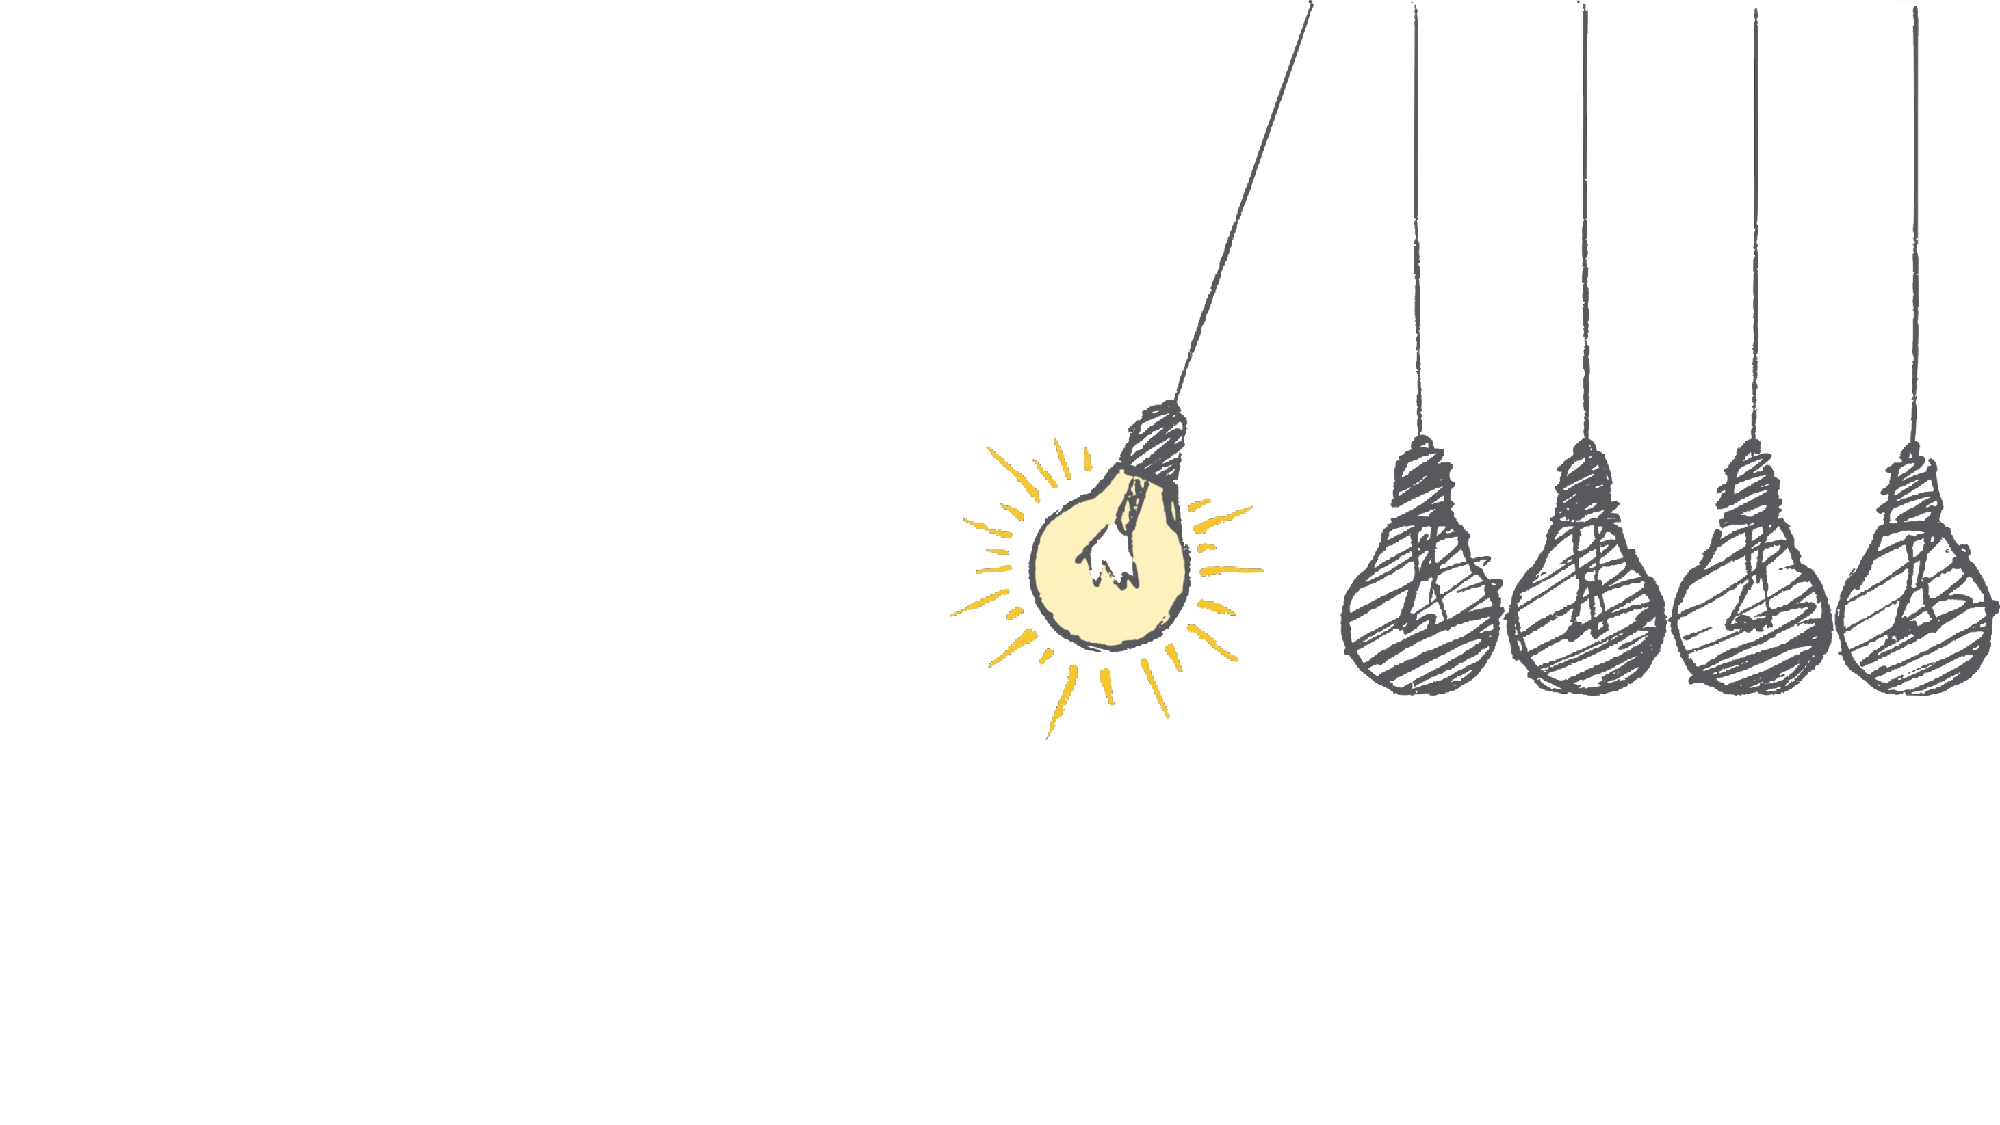
\includegraphics[height=55mm, right]{../../img/top_right_corner.pdf}}
		\maketitle
	}

%%%%%%%%%%%%%%%%%%%%%%%%%%%%%%%%%%%%%%%%%%% heading of section 1
\begin{frame}[fragile]{What are descriptive statistics?}
	\begin{columns}[c]
		\column{.5\textwidth}
		\begin{itemize}
			\item Numbers or figures that paint a picture of what a given dataset looks like
			\item They begin to help us understand the important features of our dataset, and can be useful in directing us towards areas of further analysis
			\item We will also show how to make basic regression outputs
		\end{itemize}
		\column{.5\textwidth}
		\begin{figure}
			\centering
			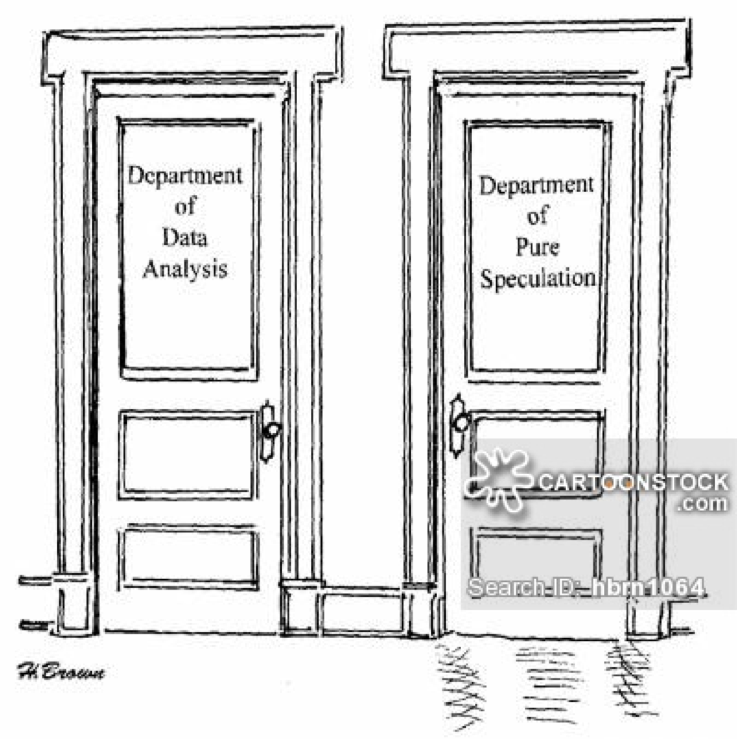
\includegraphics[width=\linewidth]{img/descriptivecartoon}
		\end{figure}
	\end{columns}
\end{frame}

\begin{frame}[fragile]{Descriptive statistics are NOT regressions}
	\begin{columns}[c]
		\column{.5\textwidth}
		\begin{itemize}
			\item This is “Anscombe’s Quartet”
			\item Every set here has:
			\begin{itemize}
				\item The same means (x and y)
				\item The same variances (x and y)
				\item The same correlation coefficient
				\item The same regression coefficient
				\item The same regression R2
			\end{itemize}
			\item Regression analysis tells you nothing about the world if you don’t understand the shape of the world you are in!
		\end{itemize}
		\column{.5\textwidth}
		\begin{figure}
			\centering
			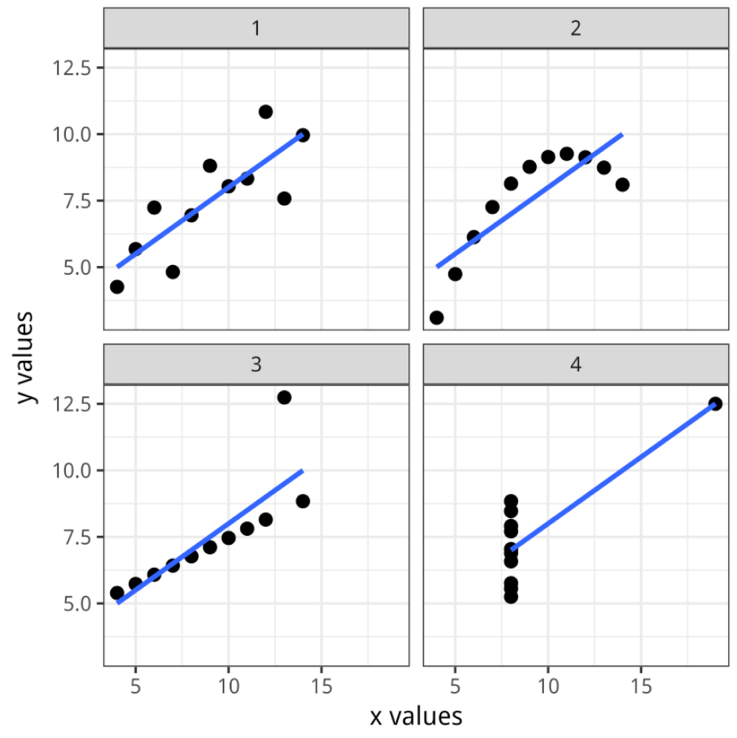
\includegraphics[width=\linewidth]{img/graphpanel1}
		\end{figure}
	\end{columns}
\end{frame}

\begin{frame}{Data can take any shape}
	\begin{figure}
		\centering
		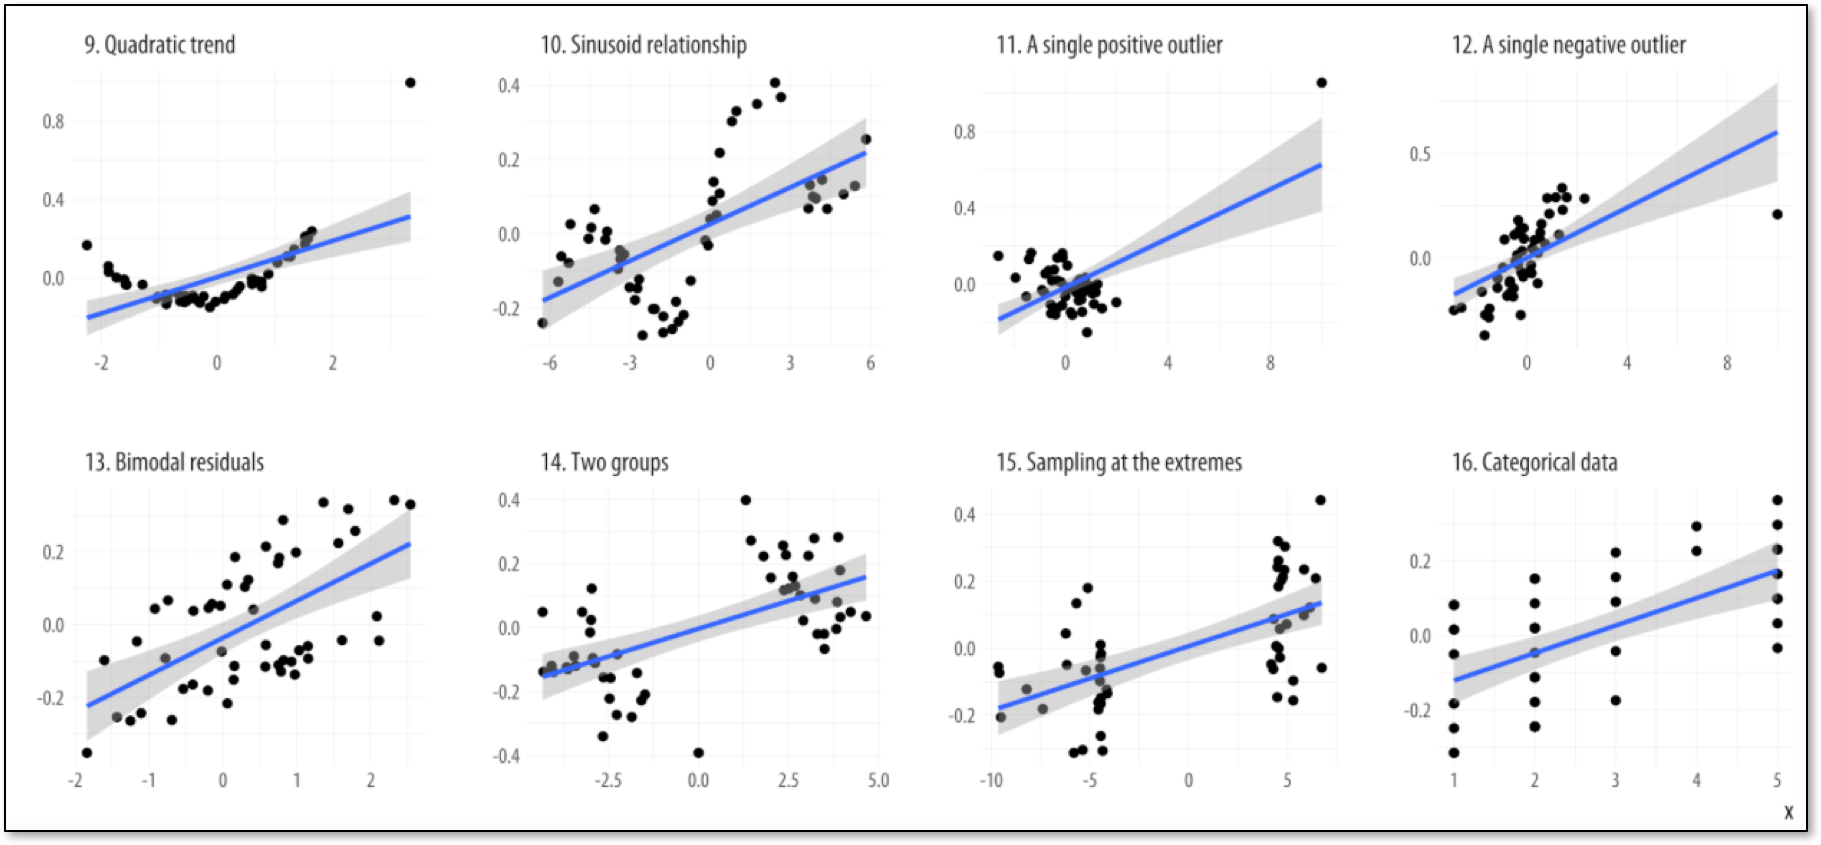
\includegraphics[width=\linewidth]{img/datashape}
	\end{figure}
\end{frame}

\begin{frame}[fragile]{This really matters for impact analysis}
	\begin{columns}[c]
		\column{.5\textwidth}
		\begin{itemize}
			\item In this case, for example, simply running a regression on the data would give a very wrong impression about the strength of the relationship
			\item And real data has many more than two dimensions!
		\end{itemize}
		\column{.45\textwidth}
		\begin{figure}
			\centering
			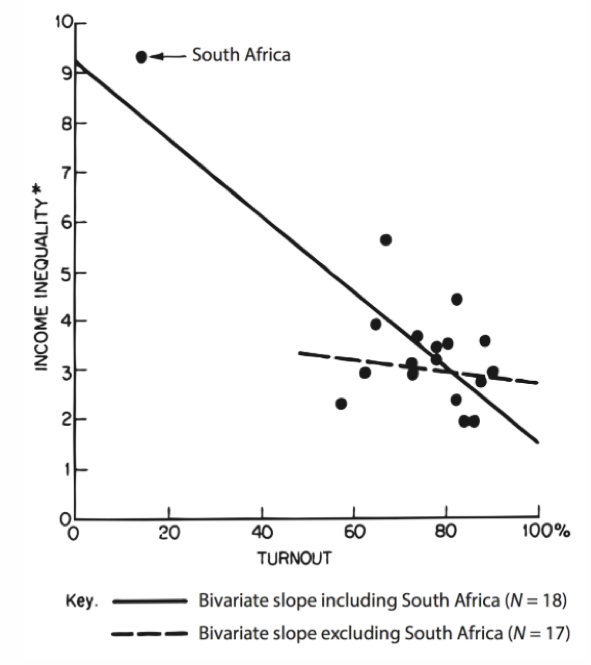
\includegraphics[width=\linewidth]{img/incomeinequality}
		\end{figure}
	\end{columns}
\end{frame}

\begin{frame}{Task 1: Summarize and Tabulate}
	\begin{itemize}
		\item These two commands are often used to get a quick idea of the data
		\item Summarize all the income variables, \texttt{inc\_01}, \texttt{inc\_02}, … \texttt{inc\_17}
		\begin{itemize}
			\item Do you see anything that stands out?
			\item Use option detail for \texttt{inc\_02}
		\end{itemize}
		\item Use tabulate to see the distribution of categorical variables
		\begin{itemize}
			\item Gender of the first person listed in the HH roster
			\item tab \texttt{pl\_sex\_1}
		\end{itemize}
	\end{itemize}
\end{frame}

\begin{frame}{Share what we learn about the data }
	\begin{itemize}
		\item \texttt{summarize} and \texttt{tabulate} are great for your quick understanding, but you need a way to share that understanding with the rest of your team
		\item \texttt{summarize} and \texttt{tabulate} do not provide a great option for this, and that is why we want to introduce some more advanced tools for that
	\end{itemize}
\end{frame}

\begin{frame}[fragile]{Three most common types of tables}
	\begin{columns}[t]
		\column{.5\textwidth}
		\begin{itemize}
			\item Summary statistics
			\begin{itemize}
				\item Show an overview of variable distributions, possible for multiple groups
			\end{itemize}
			\item Balance tests
			\begin{itemize}
				\item Show a direct comparison of variable means across treatment arms
			\end{itemize}
			\item Analysis results
				\begin{itemize}
					\item Show regression outputs in easy to read format
				\end{itemize}
		\end{itemize}

		\column{.5\textwidth}
		\begin{itemize}
			\item \texttt{sumStats}
			\begin{itemize}
				\item \url{https://github.com/worldbank/stata/tree/master/src/sumStats}
			\end{itemize}
			\item \texttt{iebaltab}
			\begin{itemize}
				\item \url{https://worldbank.github.io/ietoolkit} \newline
			\end{itemize}
			\item \texttt{estout}
			\begin{itemize}
				\item \url{http://repec.org/bocode/e/estout/esttab.html}
			\end{itemize}
		\end{itemize}
	\end{columns}
\end{frame}

\begin{frame}[fragile]{Summary statistics with [tabstat]}
	\color{red}{Do we want a prettier image?}
	\begin{columns}[c]
		\column{.5\textwidth}
		\begin{itemize}
			\item \texttt{tabstat} gives you the ability specify exactly what statistics you want in your output
			\item By default, \texttt{tabstat} only displays the mean. 
			\item We can add a whole range of statistics using the option \texttt{statistics()}. 			
		\end{itemize}
		\column{.5\textwidth}
		\begin{figure}
			\centering
			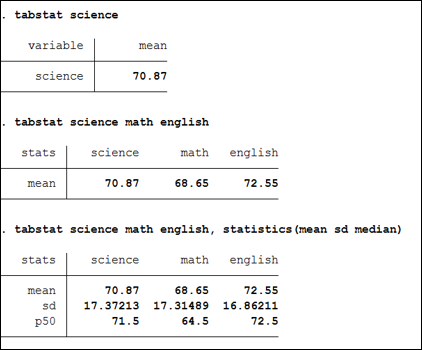
\includegraphics[width=\linewidth]{img/tabstat}
		\end{figure}
	\end{columns}
\end{frame}

\begin{frame}{Task 2 - tabstat}
	\begin{itemize}
		\item Use \texttt{tabstat} to createa a table of the mean of all income variables, \texttt{inc\_01}, \texttt{inc\_02}, … \texttt{inc\_17}
		\begin{itemize}
			\item Like this: \texttt{tabstat inc\_??}
		\end{itemize}
		\item Create a table displaying the mean, standard deviation, the median, and the number of observations for all income variables, \texttt{inc\_01}, \texttt{inc\_02}, … \texttt{inc\_17}
		\begin{itemize}
			\item Like this: \texttt{tabstat inc\_?? , statistics(mean sd median)} 
		\end{itemize}
		\item Use the help file - \texttt{help tabstat} - to try to display these statistics separately for male and female headed households
	\end{itemize}
\end{frame}


\begin{frame}[fragile]{Summary statistics with [sumStats]}
	\begin{columns}[c]
		\column{.5\textwidth}
		\begin{itemize}
			\item \texttt{sumStats} is a command that will output anything you can get from \texttt{tabstat}
			\begin{figure}
				\centering
				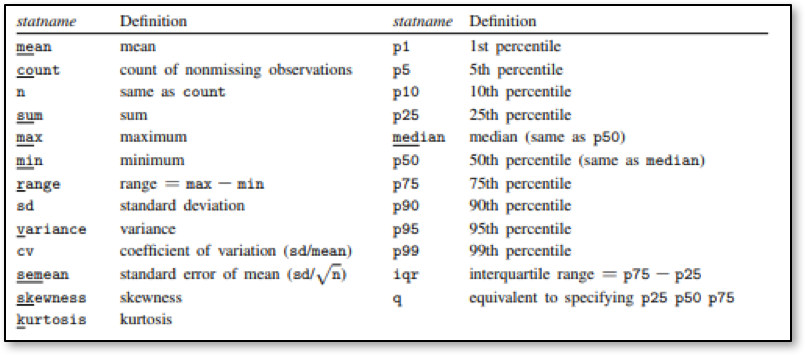
\includegraphics[width=\linewidth]{img/sumstats}
			\end{figure}
			\item It also allows multiple \texttt{if}-restrictions with different variable lists
		\end{itemize}
		\column{.5\textwidth}
		\begin{figure}
			\centering
			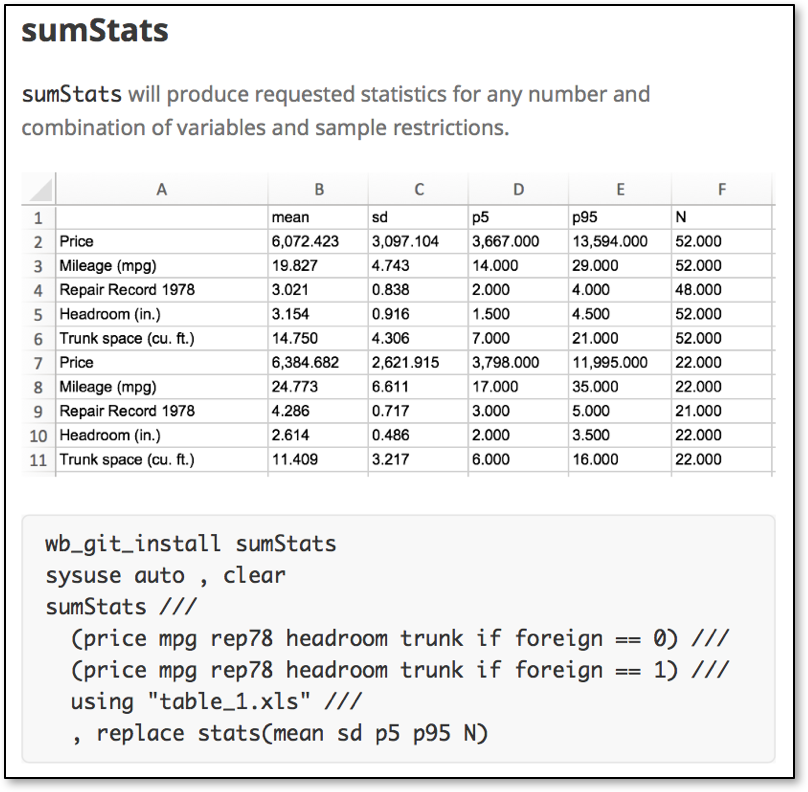
\includegraphics[width=\linewidth]{img/sumstats2}
		\end{figure}
	\end{columns}
\end{frame}



\begin{frame}{Task 3a}
	\begin{itemize}
		\item Run the code as it is in the 3a section and open the file generated. (You need to include the sections where the locals are defined)
		\begin{itemize}
			\item Only the mean is in the table
		\end{itemize}
		\item Add the two outcome locals to the varlist
		\item Add more statistics to the table. Type \texttt{help sumStats} and click the stats\_list link to see all options you can use
		\begin{itemize}
			\item Add, for example, mean, number of observation, standard deviation, median, max and min
		\end{itemize}
	\end{itemize}
\end{frame}

\begin{frame}[fragile]{Multiple levels or groups are easy}
	\begin{columns}[c]
		\column{.5\textwidth}
		\begin{itemize}
			\item Village statistics can be called with \texttt{if tag\_village == 1}
			\item Treatment group can be called with \texttt{if hh\_treatment == 1}
			\item And so on, with only one line of code in Stata
		\end{itemize}
		\column{.5\textwidth}
		\begin{figure}
			\centering
			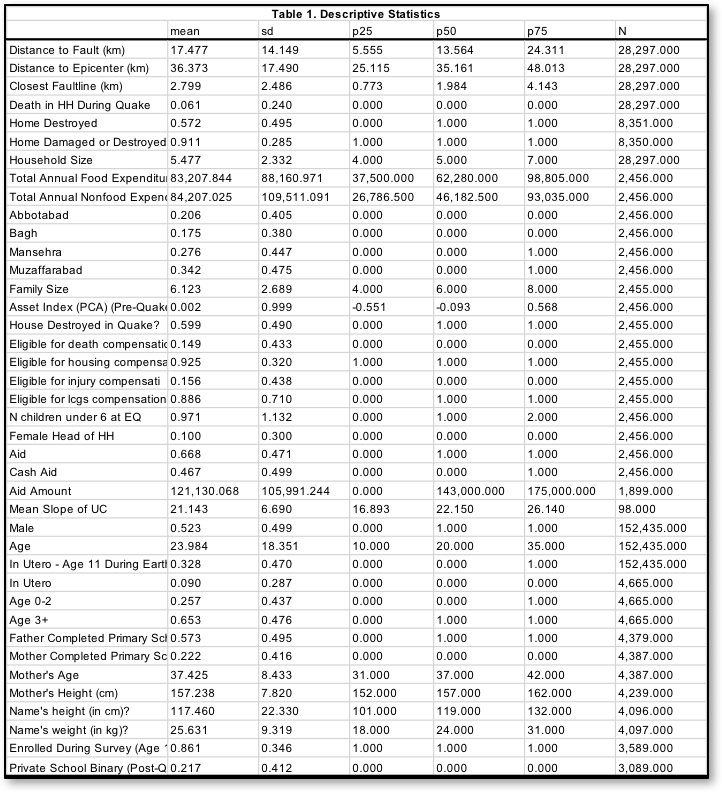
\includegraphics[width=\linewidth]{img/table1}
		\end{figure}
	\end{columns}
\end{frame}


\begin{frame}{Task 3b}
	\begin{itemize}
		\item In the Task 3b section, start by adding the outcome variables, and the additional statistics you added to the table in Task 3a
		\item Restrict the first part of the table to control observations, and the second part of the table to treatment observations
		\item Run the section for Task 3b and open the table. (Remember to include the section where the locals are defined)
	\end{itemize}
\end{frame}


\begin{frame}[fragile]{Balance tables with [iebaltab]}
	\begin{columns}[c]
		\column{.5\textwidth}
		\begin{itemize}
			\item Balance tables feature in almost every impact evaluation
			\item We use balance tables to show that there was no difference between our control and treatment group in the baseline before the intervention
			\item To use \texttt{iebaltab}, list all the variables you want to test balance in, and use the option \texttt{grpvar()} to indicate which group each observation is in.
		\end{itemize}
		\column{.5\textwidth}
		\begin{figure}
			\centering
			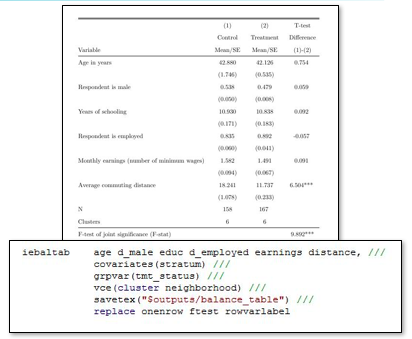
\includegraphics[width=\linewidth]{img/iedbaltab}
		\end{figure}
	\end{columns}
\end{frame}

\begin{frame}{Task 4 - Balance table}
	\begin{itemize}
		\item Run the first iebaltab section
		\begin{itemize}
			\item Click the link in the result window to see the table generated
		\end{itemize}
		\item Run the third \texttt{iebaltab} section
		\item Write some manual labels for one or a few of the income variables you added, and re-run the last \texttt{iebaltab} section again
	\end{itemize}
\end{frame}

\begin{frame}{Analysis Tables}
	\begin{itemize}
		\item Regressions are integral part of all analysis
		\item The \texttt{estout} package includes several commands which can be used to output regression results
		\item It is a 2-step process to export regression results in a presentable format using the the \texttt{estout} package
		\begin{itemize}
			\item First we store the regression results using the \texttt{eststo} command
			\item Next we export the regression results  using the \texttt{esttab} command
		\end{itemize}
	\end{itemize}
\end{frame}


\begin{frame}{Task 5: Analysis tables}
	\begin{enumerate}
		\item Install the \texttt{estout} package by typing \texttt{ssc install estout} in Stata
		\item Run the first analysis tables section
		\begin{itemize}
			\item Click the link in the result window to see the table generated
		\end{itemize}
		\item Using the help file - \texttt{help esttab} - find a way to use the variable labels instead of variable names as row names
	\end{enumerate}
\end{frame}

\begin{frame}[fragile]{Helpful checklist before sending tables to PI}
	\begin{columns}[t]
		\column{.5\textwidth}
		\begin{itemize}
			\item \scriptsize Does the number of observations for each regression or summary statistic make sense?
			\item \scriptsize Do the magnitude and sign of each coefficient/summary statistic seem reasonable?
			\item \scriptsize Did you delete the constant term and add the control mean in the regression table?
			\item \scriptsize Did you check for joint significance of your covariates?
			\item \scriptsize Did you label the dependent variables/columns?
			\item \scriptsize Did you label the covariates/rows?
			\item \scriptsize Did you add a title?
		\end{itemize}
		\column{.5\textwidth}
		\begin{itemize}
			\item \scriptsize Is it clear what the estimation procedure is (e.g. regression vs. probit)?
			\item \scriptsize Are the column widths the right size so as not to cut off text?
			\item \scriptsize Is the bordering consistent with your other tables?
			\item \scriptsize Are the numbers rounded to an appropriate level, so you don’t display too many decimal places?
			\item \scriptsize Do the notes to the table clearly indicate how standard errors have been estimated, and what control \item variables if any have been included but not shown?
		\end{itemize}
	\end{columns}
	\vspace{.1cm}
	\scriptsize  \url{https://blogs.worldbank.org/impactevaluations/generating-regression-and-summary-statistics-tables-stata-checklist-and-code}
\end{frame}

%%%%%%%%%%%%%%%%%%%%%%%%%%%%%%%%%%%%%%%%%%% Final thougts section
\begin{frame}{Conclusion}


\vspace{20mm}
For more information or further questions please contact:
\newline John Doe (\url{johndoe@worldbank.org}) \newline Mary Doe (\url{marydoe@worldbank.org})

\end{frame}

%%%%%%%%%%%%%%%%%%%%%%%%%%%%%%%%%%%%%%%%%%% The End
\sectionpic{Thank You!}{../../img/section_slide}






\end{document}
